

%=============================================================================
\section{Tool Curation Criteria}
\label{sec:tool_curation}
%=============================================================================

This section spells out the criteria used to build the \bench{} tool inventory.
The pipeline retains only tools that are executable under free-tier constraints.

\subsection{RapidAPI Endpoints}

Our RapidAPI pool is initialized from finance-related tools collected from the ToolBench paper, and then filtered with the two-stage pipeline below.

\paragraph{First-stage (rule-based) filters.}
Because RapidAPI listings vary in how authentication, billing, and rate limits are described, we programmatically crawl and parse endpoint pages to extract these fields, and then apply the deterministic criteria in Table~\ref{tab:rapidapi_filters}. An endpoint is excluded if it fails any row.


\begin{table}[h]
\centering
\caption{First-stage RapidAPI filter criteria.}
\label{tab:rapidapi_filters}
\small
\begin{tabular*}{\columnwidth}{@{}@{\extracolsep{\fill}}p{0.22\linewidth}p{0.72\linewidth}@{}}
\toprule
Criterion & Rule \\
\midrule
Description & Missing or empty $\rightarrow$ excluded. \\
Deduplication & Duplicate names: keep first only. \\
Authentication & Exclude if \texttt{Authorization} or multi-step token (beyond single API key) required. \\
Existence & Remove if endpoint does not resolve or returns persistent errors. \\
Bank-card & Exclude if free-tier requires card binding. \\
Rate limits & Require $\ge$10/h, $\ge$100/d, $\ge$300/m. \\
Map & Use an LLM to align endpoint parameter names with the tool signature and then manually spot-check the mappings. \\
\bottomrule
\end{tabular*}
\end{table}

\paragraph{Second-stage (mapping and executability).}
Each endpoint that passes the first stage is mapped into our normalized schema.
We align its parameter names to our tool signature with an LLM and then manually spot-check the mappings.
We then test each mapped endpoint with at least one successful invocation (valid request and parsed response).
Endpoints that fail consistently (timeouts, validation errors, or empty responses) are dropped.

\paragraph{Outcome.}
After the two-stage filtering process, we obtain 261 executable RapidAPI endpoints.
All retained endpoints have at least one documented required or optional parameter.
Endpoints that are parameter-free or rely solely on implicit path/query conventions are excluded.


\subsection{AkShare Interfaces}

AkShare functions are selected and then validated for executability.

\paragraph{Finance-domain filter.}
Function names are matched against a fixed set of finance-related keywords.
A function is retained if its name (or module path) contains any of the following tokens:
\begin{itemize}[leftmargin=*,nosep]
\item \texttt{stock}, \texttt{fund}, \texttt{bond}, \texttt{futures}, \texttt{option}, \texttt{index}, \texttt{macro}, \texttt{currency}, \texttt{fx}, \texttt{crypto}, \texttt{rate}, \texttt{treasury}, \texttt{etf}
\item \texttt{finance}, \texttt{bank}, \texttt{insurance}, \texttt{security}, \texttt{derivative}, \texttt{swap}, \texttt{gold}, \texttt{commodity}, \texttt{interest}, \texttt{libor}, \texttt{shibor}, \texttt{exchange}, \texttt{margin}
\end{itemize}

\paragraph{Executability.}
Each candidate is invoked with minimal valid arguments, using defaults or small example values where possible.
Interfaces that raise import errors, signature errors, or runtime errors under a timeout are discarded.

\paragraph{Outcome.}
After finance-domain filtering and executability validation, we retain 499 AkShare interfaces in the final tool inventory.

\subsection{Combined Inventory}

After executability filtering, the final tool library contains 760 tools.
All tools in \bench{} are normalized into a single manifest schema, including tool name, description, and parameters.
This unified manifest enables auditable tool traces and call-level compliance metrics (TMR, IMR, DMR), where each run records the invoked tools together with their arguments and execution outcomes.


%=============================================================================
\section{Finance Attribute Schema and Labeling}
\label{sec:attributes}
%=============================================================================

Each tool is annotated with finance attributes that make timeliness, intent, and domain constraints explicit.
These attributes support both tool cards (for planning) and compliance evaluation (TMR, IMR, DMR).

\subsection{Attributes of the Tools}

\begin{itemize}[leftmargin=*]
\item \textbf{Timeliness} (\texttt{timeliness}): one of\\
  \realt, \dailyt, \asfiledt, \periodict, or \statict.
  \begin{itemize}[nosep]
  \item \realt: intra-day, low latency, such as ticks and order book.
  \item \dailyt: updated once per trading day or batch, such as closing prices and NAV.
  \item \asfiledt: event-driven, when a regulated entity files, such as filings and announcements.
  \item \periodict: fixed calendar schedule, such as quarterly reports and GDP.
  \item \statict: rarely changes, such as identifiers and listing dates.
  \end{itemize}
\item \textbf{Intent type} (\texttt{intent\_\allowbreak type}): one of\\
  \informational, \advisory, or \transactional.
  \begin{itemize}[nosep]
  \item \informational: read-only data access and factual retrieval without recommendations or actions.
  \item \advisory: analysis or recommendation-oriented outputs that go beyond pure retrieval.
  \item \transactional: action-triggering operations such as order placement, transfer, or account-changing behavior.
  \end{itemize}
\item \textbf{Regulatory domain} (\texttt{regulatory\_\allowbreak domain}):\newline
  Subset of \{equity, bond, fund, forex, derivatives, macro,\\ economic\_\allowbreak policy, sentiment\_\allowbreak trading, esg, crypto\}. Multiple values are allowed per tool.
\end{itemize}

\subsection{Labeling Protocol}

Annotations are produced by an LLM (Qwen3-8B) given the tool name and description.
Each attribute is labeled independently with three samples, and the final label is the majority vote.
This protocol keeps labeling separate from the agent under test and makes the compliance layer auditable.

%=============================================================================
\section{Question Set Construction}
\label{sec:questions}
%=============================================================================

The question set is built so that every retained question requires tool use.
Questions answerable by static memorization or general reasoning are excluded.

\subsection{Sources}

Questions are drawn from the FinanceBench release and the OpenFinData release (dataset identifier \texttt{openfindata\_}\allowbreak\texttt{release}).
Only questions that require tool calls to answer are retained, such as current prices, time series, or structured data.

\subsection{Filters}

\begin{itemize}[leftmargin=*,nosep]
\item \textbf{Standardization:} Convert all sources into a unified \texttt{\{question, answer, category\}} format.
\item \textbf{Maximum length:} 500 characters to keep prompts within a fixed budget.
\item \textbf{Candidate retrieval:} For each question, retrieve Top-$K$ tools ($K{=}20$) using BGE-M3 embeddings.
\item \textbf{LLM tool selection:} Given the Top-$K$ tools, Qwen3-8B selects the most suitable tool(s). We sample three times and keep tools with at least two votes.
\item \textbf{Deduplication:} For single-tool questions, keep at most two questions per tool to reduce skew. Multi-tool questions are not deduplicated by tool set.
\end{itemize}

\subsection{Outcome}

The final question set contains 295 questions, spanning both simple and compositional tool use: 166 single-tool questions and 129 multi-tool questions, classified by the number of tool calls observed at runtime.

%=============================================================================
\section{Metric Definitions}
\label{sec:metrics}
%=============================================================================

All metrics are defined over a fixed question set and a fixed evaluation protocol (timeout, retries, caching).
We report capability (TIR, TESR, CER) and compliance (TMR, IMR, DMR) to separate whether an agent can run tools from whether its tool choices satisfy finance constraints.
Below, $N$ denotes the number of questions.

\subsection{Capability}

\begin{itemize}[leftmargin=*]
\item \textbf{Tool Invocation Rate (\tir).} Fraction of questions whose execution invokes at least one tool call:
\[\mathrm{TIR}=\frac{1}{N}\sum_{i=1}^{N}\mathbf{1}\!\left[\,|\mathrm{tool\_calls}_i|>0\,\right].\]
\item \textbf{Tool Execution Success Rate (\tesr).} Fraction of questions whose tool execution succeeds.
We mark a question successful when its final tool call returns a valid parsed output without error or exception; intermediate failures and retries are allowed:
  \[\mathrm{TESR}=\frac{1}{N}\sum_{i=1}^{N}\mathbf{1}\!\left[\,\text{final tool call succeeds on question } i\,\right].\]
\item \textbf{Conditional Execution Rate (\cer).} Success rate among questions that invoked at least one tool call: 
  \[\mathrm{CER}=\frac{\mathrm{TESR}}{\mathrm{TIR}},\quad \mathrm{CER}=0 \text{ when } \mathrm{TIR}=0.\]
\item \textbf{Soft Score (\soft).} 
We partition questions into three types based on the gold-answer format:
(i) numeric/choice questions, identified by the presence of a \texttt{numeric} or \texttt{choices} field in the gold answer;
(ii) structured-analysis questions, identified by the presence of a \texttt{criterium} field in the gold answer;
(iii) \texttt{other} questions, all remaining non-numeric/choice/\texttt{criterium} cases.
All questions are judged by LLM (GPT-5.1). Numeric/choice questions are scored in $\{1,0\}$, while structured-analysis and \texttt{other} questions are scored in $\{1,0.5,0\}$. Scores are averaged over three judging repeats.
\[\mathrm{SoftScore}=\frac{1}{3N}\sum_{i=1}^{N}\sum_{r=1}^{3} s_{i,r}.\]
\item \textbf{Conditional Soft Score (\css).} Mean \soft{} over questions with successful execution:
  \[\mathrm{CSS}=\frac{\mathrm{Soft\ Score}}{\mathrm{TESR}},\quad \mathrm{CSS}=0 \text{ when } \mathrm{TESR}=0.\]
\end{itemize}



\subsection{Compliance Mismatch Rates}

For each question $q$, an LLM(GPT-5.1) judge assesses whether the tools used in the execution are aligned with the question's finance constraints in timeliness, intent type, and regulatory domain.
Let the executed tool-use trace be $\tau=\{(t_k,x_k,o_k)\}_{k=1}^{m}$, where $t_k$ is the tool name selected at step $k$, $x_k$ is the tool input (arguments), and $o_k$ is the tool output.
Tool attributes are not part of the trace; instead, for any tool $t$ we look up its finance tags from the tool metadata:
$A(t)=(t(t), i(t), d(t))$, corresponding to timeliness $t(t)$, intent type $i(t)$, and regulatory domains $d(t)$.

Define judge-level call alignment indicators:
$J_T(q,t_k,x_k,o_k,T(t_k))\in\{0,1\}$,
$J_I(q,t_k,x_k,o_k,I(t_k))\in\{0,1\}$,
and $J_D(q,t_k,x_k,o_k,D(t_k))\in\{0,1\}$,
where $1$ means matched and $0$ means mismatched.
We then define mismatch-at-least-once indicators at the question level:
\begin{align*}
\mathrm{TMR}(q,\tau) &= \mathbf{1}\!\left[\exists k:\ J_T(q,t_k,x_k,o_k,T(t_k))=0\right], \\
\mathrm{IMR}(q,\tau) &= \mathbf{1}\!\left[\exists k:\ J_I(q,t_k,x_k,o_k,I(t_k))=0\right], \\
\mathrm{DMR}(q,\tau) &= \mathbf{1}\!\left[\exists k:\ J_D(q,t_k,x_k,o_k,D(t_k))=0\right].
\end{align*}

TMR, IMR, and DMR count the number of questions whose traces contain at least one mismatched tool call in the corresponding dimension.
Each question is counted once, regardless of how many mismatches occur in its trace.
We report these metrics as rates in $[0,1]$ by dividing the mismatch count by the number of questions that invoked at least one tool call.
Lower is better.



%=============================================================================
\section{Prompt Templates}
\label{sec:prompt_templates}
%=============================================================================

This section documents the prompts for (i) intent mismatch evaluation, (ii) planner system instructions, and (iii) RapidAPI Parameter Alignment.

\subsection{Intent-Match Evaluator (IMR)}

We use an LLM(GPT-5.1) judge to decide whether a tool call's \texttt{intent\_type} is compatible with the question requirement.
The judge considers only intent (informational, advisory, transactional) and ignores execution success.

\begin{promptcard}{Intent match prompt (JSON-only output)}
You are a financial tool compliance evaluator. Determine whether the "question requirement" matches the "tool intent".\\
Consider only tool intent. Do not consider whether the tool call succeeds.\\
Tool intent must be one of \texttt{informational} / \texttt{advisory} / \texttt{transactional}.

Question: \{question\}\\
Tool name: \{tool\_name\}\\
Tool intent (\texttt{intent\_type}): \{tags.get("intent\_type")\}\\
Tool description: \{tags.get("description") or ""\}

Output JSON only:
\{
  "match": "yes|no",
  "reason": "within 20 words"
\}
\end{promptcard}

\subsection{Planner System}

The planner is explicitly instructed to use the \texttt{financial\_tags} field inside each tool description when choosing tools.
This makes timeliness, domain, and intent cues salient at selection time.

\begin{promptcard}{Planner system}
% You can see the \texttt{financial\_tags} field in tool descriptions.\\
% When selecting tools, use these attributes to help your decision, including the tool's timeliness, regulatory domain, and compliance risk.\\
% Subject to satisfying the question, prefer tools with appropriate timeliness whose domain and intent better match the requirement.
Subject to satisfying the question, first infer the question’s required finance tags:
(a) required \texttt{timeliness}, (b) required \texttt{regulatory\_domains}, and (c) allowed \texttt{intent\_type}.\\
Then select tools whose \texttt{financial\_tags} best match these requirements: require domain overlap, prefer matching timeliness, and choose the lowest-risk intent (\texttt{informational} > \texttt{advisory}; avoid \texttt{transactional} unless explicitly requested).\\
If multiple tools match, choose the one whose signature/description best fits the needed inputs/outputs.
\end{promptcard}

\subsection{RapidAPI Parameter Alignment}

RapidAPI documentation often uses parameter names that differ from those used in request examples.
To reduce argument instantiation errors, we generate normalized Python wrappers whose function parameters exactly match the keys used in the request schema, and we verify mappings with manual spot-checking (Table~\ref{tab:rapidapi_filters}, Map rule).
For security, we show the API key as a placeholder.

\begin{promptcard}{Parameter-aligned Python code generation prompt}
You are a professional Python tool function generator. Rewrite the following raw API call code into a standard reusable function.\\
Strictly follow the rules below.\par

1. Function name: \{func\_name\}\\
2. Function parameters:\par
- All input parameters: \{param\_str\}\\
- Additional fixed parameter: \texttt{rapidapi\_key: str = "<RAPIDAPI\_KEY>"}\par
3. The function must:\par
- Use \texttt{requests} to send the HTTP request\\
- Use \texttt{X-RapidAPI-Key} and \texttt{X-RapidAPI-Host} in headers\\
- Return \texttt{response.json()} if possible, otherwise return \texttt{response.text}\\
% - Do not use \texttt{print}. Always \texttt{return}\\
% - Include a full docstring describing the function and every parameter\\
- Do not explain anything. Output pure Python code only\\
- Parameter names must exactly match the keys in the parameter dictionary (case sensitive)\par

Description: \{desc\}\\
Parameter spec: \{parameters\}\par
URL:\{url\}\par
X-RapidAPI-Host:\{url.split('/')[2]\}\par

\end{promptcard}


%=============================================================================
\section{Commands and Reproduction Checklist}
\label{sec:commands}
%=============================================================================

The following enables independent reproduction of the benchmark and evaluation pipeline so that results can be compared fairly across studies.

\subsection{Environment and Models}

RapidAPI keys are obtained following the official documentation. AkShare usage follows its documentation.
Retriever: BGE-M3. Planner: exact model names and versions, for example Doubao-Seed-1.6, Qwen3-8B, and GLM-4.7-Flash, plus inference hyperparameters (temperature, max tokens).
Judge: GPT-5.1 (3 repeats) for \soft{} and requirement metrics. Record these identifiers in the repository \texttt{README} or a config file so that tables in the paper can be reproduced.

%=============================================================================

\section{Algorithm --- FATR Pipeline}
\label{sec:algorithm}
%=============================================================================

\begin{algorithm}[H]
\caption{FATR pipeline}
\begin{algorithmic}[1]
\Require Question $q$, tool library $\mathcal{T}$, retriever $\mathcal{R}$, planner LLM $\pi$, Top-$K$ (default $K{=}20$)
\Ensure Final answer $\hat{y}$, tool trace $\tau$
\State $\mathcal{C} \gets \mathcal{R}(q, \mathcal{T}, K)$ \Comment{Retrieve Top-$K$ tools by similarity}
\State Build tool cards: for each $t \in \mathcal{C}$, format $\mathrm{Card}(t)$ with signature and finance attributes
\State $\tau \gets \emptyset$, $h \gets \emptyset$ \Comment{History of tool calls and outputs}
\Repeat
\State Planner $\pi$ proposes next action given $(q,\{\mathrm{Card}(t)\}_{t\in\mathcal{C}},h)$: tool $t$ and arguments $x$ (or final answer $\hat{y}$)
\If{action is tool call $(t, x)$}
\State Validate $t \in \mathcal{C}$
\State Execute: $o \gets \mathsf{Exec}(t, x)$ with timeout, optionally compress $o$
\State Append $(t, x, o)$ to $\tau$, update $h$ with observation
\Else
\State $\hat{y} \gets$ planner output, \textbf{break}
\EndIf
\Until{planner emits final answer or max steps}
\State \Return $\hat{y}$, $\tau$
\end{algorithmic}
\end{algorithm}
\FloatBarrier



The algorithm in this section summarizes the \methodname{} pipeline: retrieval, tool-card formatting, ReAct-style planning with finance constraints, and stabilized execution (timeout, retries, cache, optional output compression).
When output compression is enabled, we use Qwen3-8B as the extractor to keep only question-relevant fields from long tool responses.
This algorithm serves as the reference implementation for the \methodname{} baseline in the main paper.

% Attribute injection ablation is reported in the main paper (Section~\ref{sec:experiments}).

%============================================================================
\section{Category-Level Diagnosis}
\label{sec:category_diagnosis}
%=============================================================================

To further localize failure modes beyond aggregate averages, we report metrics broken down by question category.
Figure~\ref{fig:metrics_by_category} presents category-level performance for Doubao-Seed-1.6.
The heatmap highlights substantial heterogeneity across categories.
Categories with low \tir cap end-to-end execution success by limiting tool coverage.
In contrast, categories with high \tir but low \tesr indicate difficulties in argument construction, disambiguation, or endpoint instability even after the agent commits to tool use.

\begin{figure*}[!tb]
\centering
% 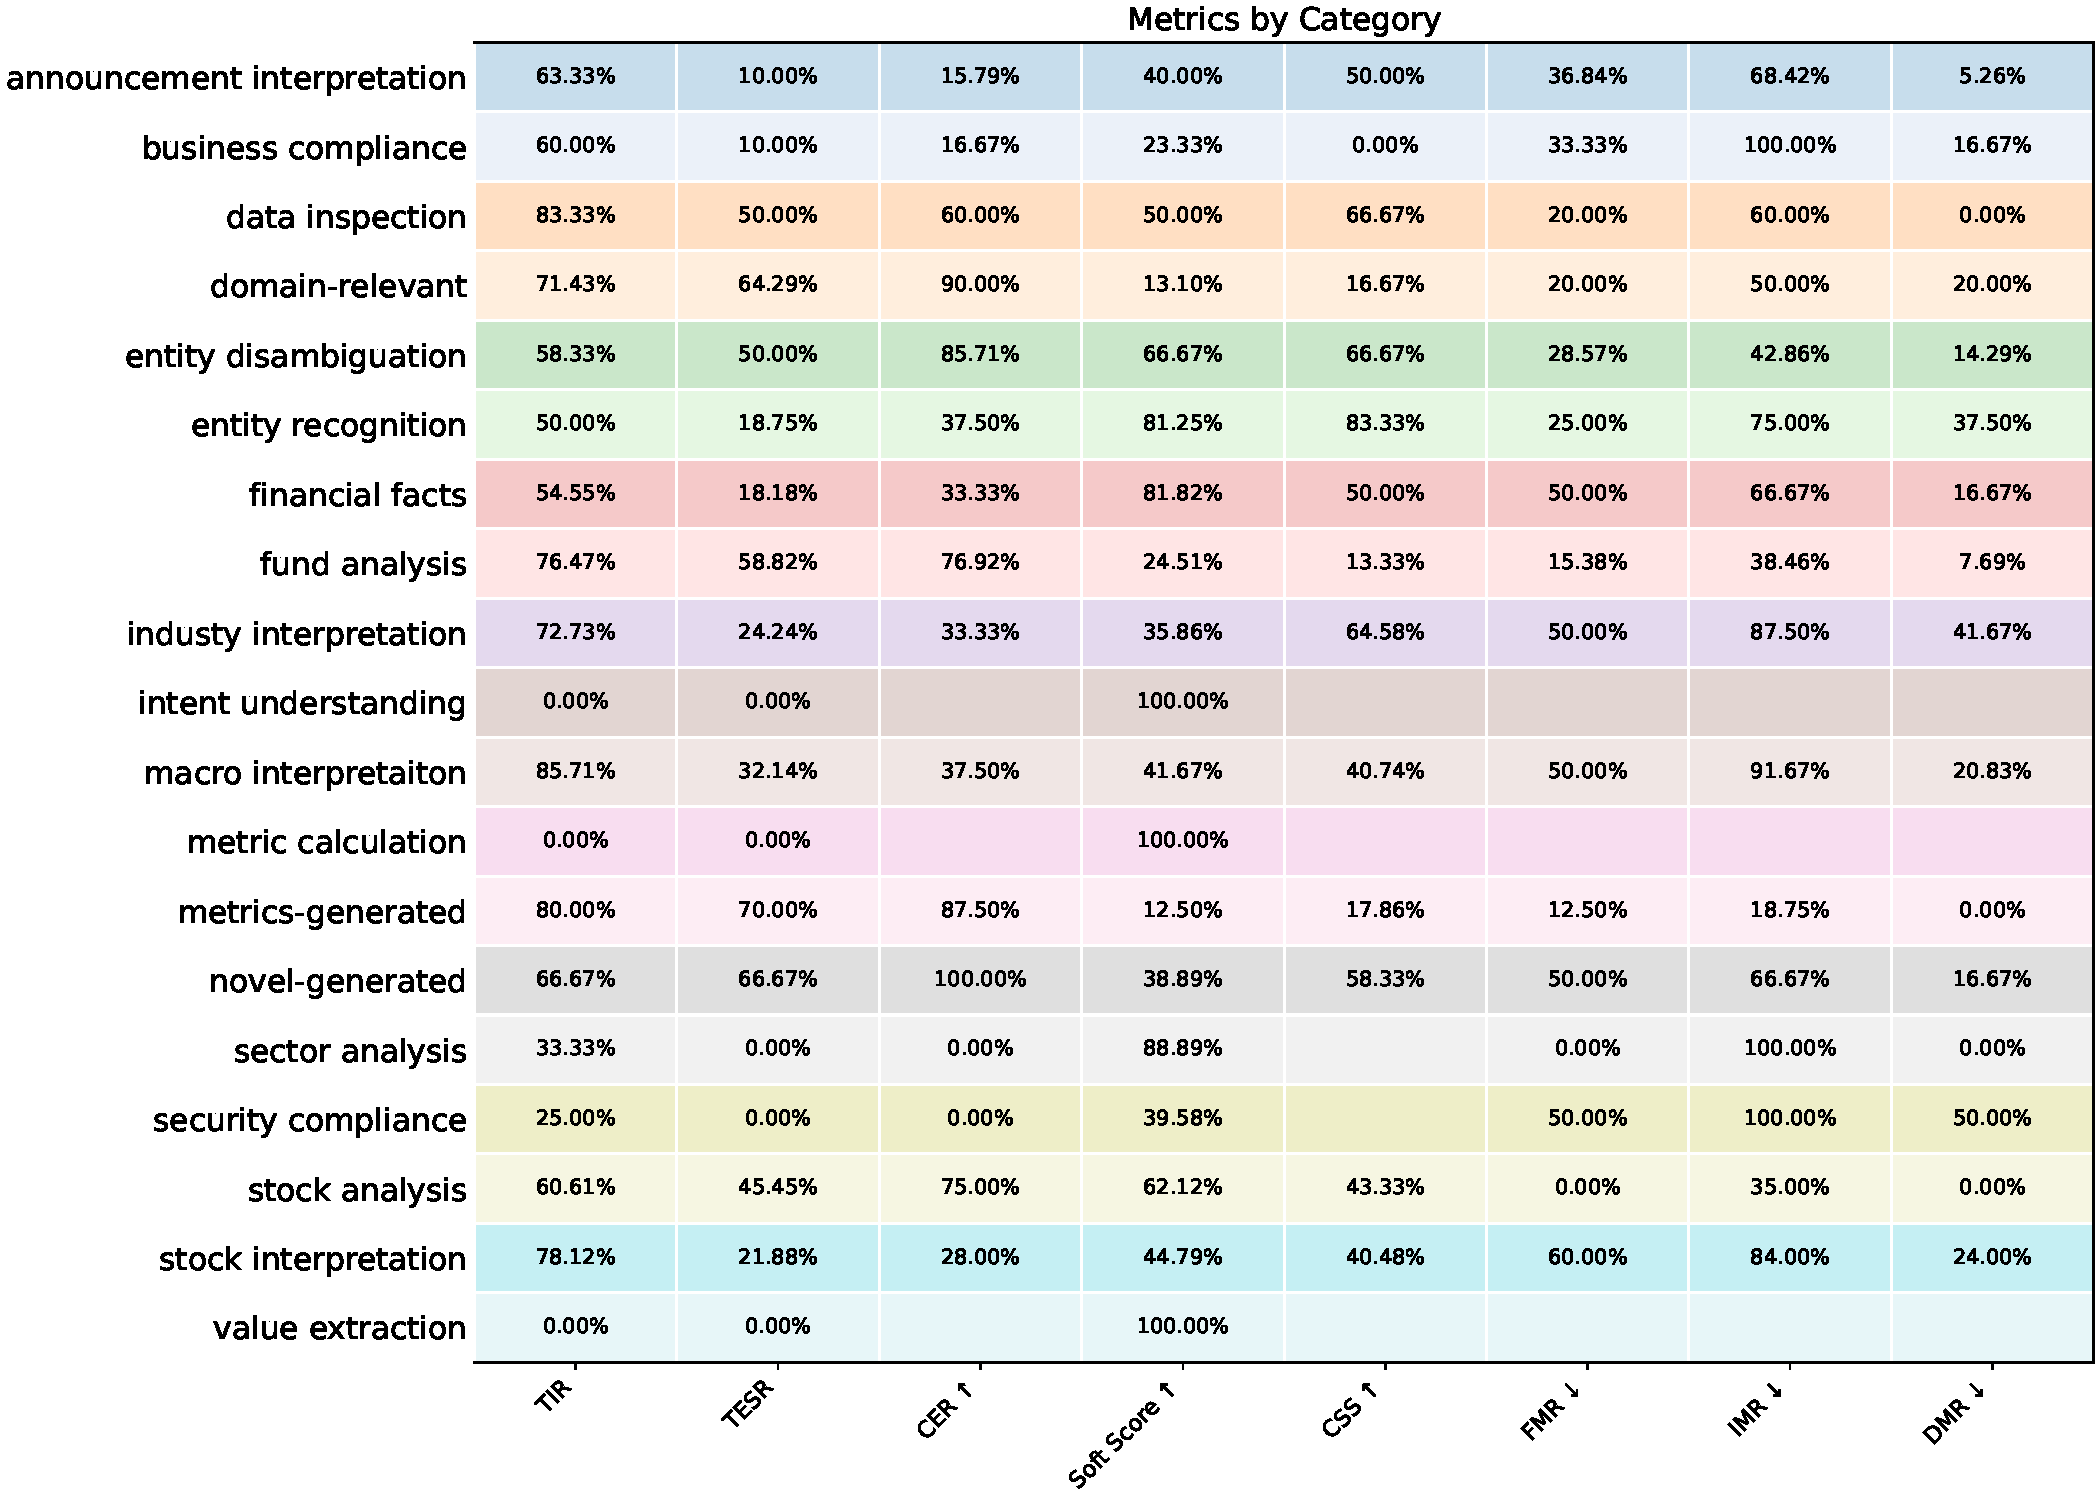
\includegraphics[width=\textwidth]{result_Doubao-Seed-1.6_full_by_category.pdf}
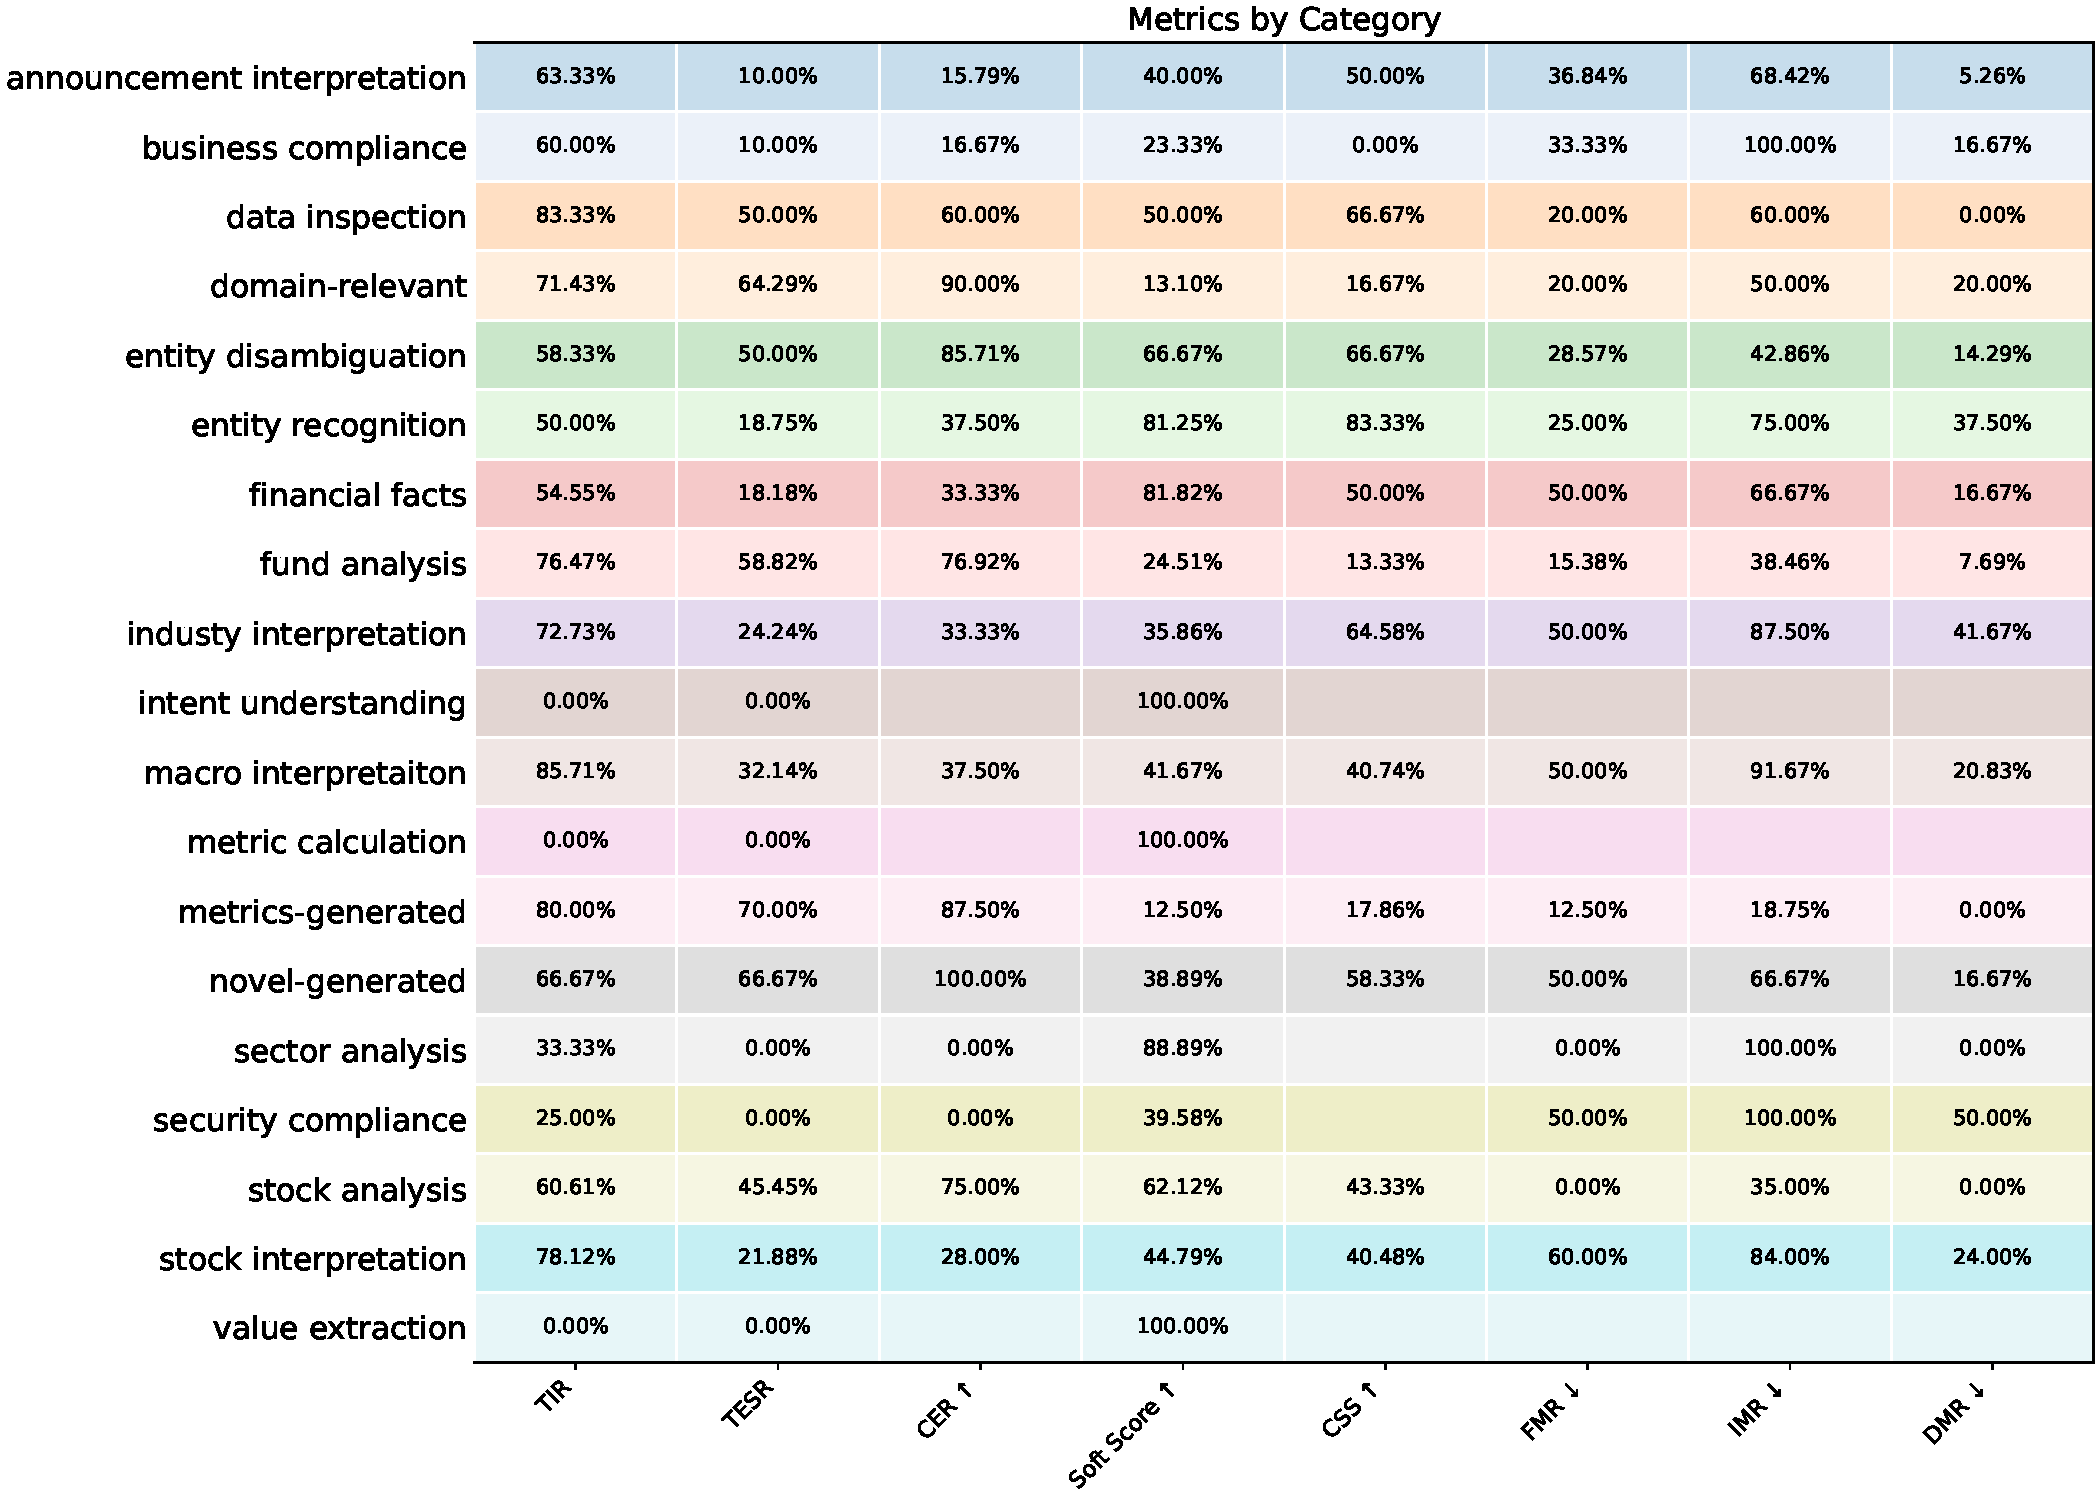
\includegraphics[scale=0.38]{result_Doubao-Seed-1.6_full_by_category.pdf}
\caption{Metrics by category for Doubao-Seed-1.6 on FinToolBench. Rows are question categories and columns are evaluation metrics.}
\Description{Heatmap of FinToolBench metrics by category for Doubao-Seed-1.6.}
\label{fig:metrics_by_category}
\end{figure*}

%=============================================================================



%=============================================================================
\section{Case Studies}
\label{sec:case_studies}
%=============================================================================

This section presents representative end-to-end execution traces from our evaluation logs.
Each case study reports the full question, the agent's tool calls (with condensed outputs),
the final answer, correctness against dataset ground truth, and an analysis highlighting
what the trace reveals about agentic financial tool use.

%=============================================================================
\subsection{Case Study 1: Finance Attribute Injection Changes Tooling Behavior}
\label{sec:case_study_financebench_margin}
%=============================================================================

This case examines whether finance-attribute injection changes tool-selection behavior
when the first attempted interface is partially incompatible with the benchmark wrapper.
We compare a baseline planner (without attribute tags in tool cards) against \methodname{}
under the same retrieval pool and execution budget. The key question is not only whether
the run finishes, but whether the resulting trace supports the dataset's intended reasoning target.

\begin{figure*}[htbp]
\begin{casecard}{Case Study 1 (\texttt{financebench\_9}): injection recovers tool execution but not task framing}
\textbf{Question.} Does AMEX have an improving operating margin profile as of 2022? If operating margin is not a useful metric for a company like this, then state that and explain why.\par
\smallskip
\textbf{Ground truth.} ``Performance is not measured through operating margin.''\par
\medskip
\begin{minipage}[t]{0.49\textwidth}
\textbf{Baseline (no finance attributes).}\par
\textbf{Tool trace.}\par
Step 1: \texttt{symbols\_get\_fundamentals} $\rightarrow$ error (unexpected keyword argument \texttt{fields}).\par
\textbf{Final answer.} No final answer is produced.\par
\textbf{Correctness.} Incorrect or unscored.\par
\end{minipage}\hfill
\begin{minipage}[t]{0.49\textwidth}
\textbf{\methodname{} (with injected finance attributes).}\par
\textbf{Tool trace.}\par
Step 1: \texttt{symbols\_get\_fundamentals} $\rightarrow$ empty.\par
Step 2: \texttt{symbols\_get\_sector\_metrics} $\rightarrow$ single-period margin.\par
Step 3: \texttt{symbols\_get\_fundamentals} (\texttt{limit=3}) $\rightarrow$ empty.\par
Step 4: \texttt{symbols\_financials\_metrics} $\rightarrow$ FY22 operating income grows slower than revenue.\par
\textbf{Final answer.} AMEX’s operating margin did not improve in 2022; revenue outpaced operating income.\par
\textbf{Correctness.} Incorrect.\par
\end{minipage}
\medskip

\textbf{Analysis.} Finance attributes change tooling behavior. The injected run recovers from early API-interface failures and produces a tool-backed narrative, while the baseline fails to complete a trace. However, correctness still depends on aligning with the dataset's intended criterion. Here, the tool-backed answer discusses margin trends instead of adopting the ground-truth stance that operating margin is not the right performance metric.\par
\end{casecard}
\caption{Single-box, end-to-end comparison for \texttt{financebench\_9}. The baseline fails due to an interface mismatch. \methodname{} recovers a valid tool trace, but the final answer remains incorrect because it does not follow the dataset's intended reasoning criterion.}
\label{fig:case_study_financebench_margin}
\end{figure*}

\paragraph{Takeaway.}
Attribute injection improves execution continuity (the agent keeps searching for viable tools after early failures),
but it does not by itself guarantee semantic alignment with the benchmark intent.
In this item, the injected run is operationally stronger but still judged incorrect because
the final reasoning criterion diverges from the annotated ground-truth stance.
This trace-level pattern is illustrated in Figure~\ref{fig:case_study_financebench_margin}.

%=============================================================================
\subsection{Case Study 2: Finance Attributes Reduce Redundant Tooling}
\label{sec:case_study_openfindata_fund}
%=============================================================================

This case focuses on trace efficiency rather than final-answer difficulty.
The question can be answered with one fund-specific informational endpoint,
so extra calls mostly reflect planner uncertainty or weak tool prioritization.
We use this example to show how finance tags can suppress unnecessary exploration.

\begin{figure*}[htbp]
\begin{casecard}{Case Study 2 (\texttt{openfindata\_release\_155}): injection prunes redundant tools while preserving correctness}
\textbf{Question.} As a financial analyst, evaluate the downside risk profile of the Tianhong Yu'e Bao Money Market Fund using the downside risk data provided below.\par
\smallskip
\textbf{Ground truth.} Tianhong Yu'ebao has a low downside risk and is among the better performers in its category.\par
\medskip
\begin{minipage}[t]{0.49\textwidth}
\textbf{Baseline (no finance attributes).}\par
\textbf{Tool trace.}\par
\texttt{fund\_individual\_analysis\_xq} $\rightarrow$ volatility metrics inconsistent with money funds.\par
\texttt{fund\_money\_fund\_info\_em} $\rightarrow$ timeout or serialization error.\par
\texttt{rate\_interbank} $\rightarrow$ execution error.\par
\texttt{fund\_overview\_em} $\rightarrow$ confirms low downside risk.\par
\textbf{Final answer.} Tianhong Yu'e Bao Money Market Fund exhibits extremely low downside risk, significantly below the peer average, making it suitable for conservative investors.\par
\textbf{Correctness.} Correct.\par
\end{minipage}\hfill
\begin{minipage}[t]{0.49\textwidth}
\textbf{\methodname{} (with injected finance attributes).}\par
\textbf{Tool trace.}\par
\texttt{fund\_overview\_em} $\rightarrow$ confirms near-zero downside risk.\par
\textbf{Final answer.} Over the past year and across multiple short-term horizons, Tianhong Yu'e Bao Money Market Fund exhibits near-zero downside risk, significantly outperforming the peer average.\par
\textbf{Correctness.} Correct.\par
\end{minipage}
\medskip

\textbf{Analysis.} Injection improves trace quality by pushing the planner toward a fund-specific, informational tool with appropriate scope. The baseline eventually reaches a suitable tool, but only after several failed or ill-suited calls. In this qualitatively straightforward item, both runs are correct, so the benefit mainly appears as a cleaner and more stable execution trace.\par
\end{casecard}
\caption{Single-box comparison for \texttt{openfindata\_release\_155}. Injected finance attributes reduce redundant and incompatible tool calls while preserving correctness.}
\label{fig:case_study_openfindata_fund}
\end{figure*}

\paragraph{Takeaway.}
Both runs are correct, but the injected run reaches the answer with a shorter and cleaner trace.
This demonstrates that finance attributes can improve practical reliability by reducing avoidable calls and failures,
even when end-task correctness is unchanged.
This efficiency-oriented gain is illustrated in Figure~\ref{fig:case_study_openfindata_fund}.

%=============================================================================
\subsection{Case Study 3: Finance Attributes Do Not Guarantee Numerical Fidelity}
\label{sec:case_study_financebench_cogs}
%=============================================================================

This case isolates a harder failure mode: the required numeric target is not directly exposed by the
available tool outputs in a straightforward way, and the planner must choose between abstaining and
using a proxy. We compare how baseline and injected settings handle this under identical constraints.

\begin{figure*}[!t]
\begin{casecard}{Case Study 3 (\texttt{financebench\_33}): injection changes strategy but remains incorrect}
\textbf{Question.} What is Nike's three-year average cost of goods sold as a percentage of revenue from FY2016 to FY2018?\par
\smallskip
\textbf{Ground truth.} 55.1\%.\par
\medskip
\begin{minipage}[t]{0.49\textwidth}
  
\textbf{Baseline (no finance attributes).}\par
\textbf{Tool trace.}\par
Income-statement tools $\rightarrow$ historical data locked or unavailable.\par
\texttt{stock\_get\_cost\_of\_revenue} $\rightarrow$ single-point value without year context.\par
\textbf{Final answer.} The requested three-year average cannot be calculated with the available data.\par
\textbf{Correctness.} Incorrect.\par
\end{minipage}\hfill
\begin{minipage}[t]{0.49\textwidth}
\textbf{\methodname{} (with injected finance attributes).}\par
\textbf{Tool trace.}\par
\texttt{symbols\_get\_sector\_metrics} $\rightarrow$ gross margin retrieved.\par
\textbf{Final answer.} Using gross margin (38.6\%), the implied average COGS ratio is approximately 61.4\%.\par
\textbf{Correctness.} Incorrect.\par
\end{minipage}
\medskip

\textbf{Analysis.} Injection pushes the agent away from unavailable historical statements toward a proxy metric. This avoids dead ends, but it does not ensure numerical fidelity. Even with a cleaner trace, the agent can still produce an incorrect estimate when the required quantity is not directly supported by the available tools.\par
\end{casecard}
\caption{Single-box comparison for \texttt{financebench\_33}. Injected finance attributes change the tool strategy, but the resulting proxy-based estimate remains incorrect.}
\label{fig:case_study_financebench_cogs}
\end{figure*}



\paragraph{Takeaway.}
Finance attributes can redirect the planner to a more plausible tool path, but they are not a substitute
for numeric-grounding checks. When only proxy signals are available, a trace may look coherent and still
produce quantitatively wrong conclusions.
This failure mode is illustrated in Figure~\ref{fig:case_study_financebench_cogs}.
